\providecommand{\main}{../../..}
\documentclass[\main/dresen_thesis.tex]{subfiles}

\begin{document}
  \subsection{D22}\label{ch:lss:d22}
    \begin{figure}[ht]
      \centering
      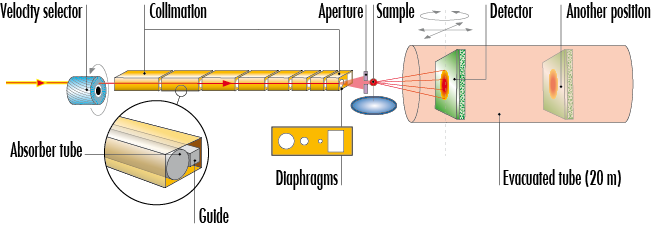
\includegraphics[width=0.7\textwidth]{appendix_instruments_d22Setup}
      \caption{\label{fig:lss:d22}D22 instrument at Institut Laue-Langevin used for small angle scattering with (polarized) neutrons (schematics reproduced from \cite{Porcar_2018_D22La}).}
    \end{figure}
    D22 \cite{Porcar_2018_D22La} is small-angle diffractometer at the Institut Laue-Langevin equipped for the measurement of polarized neutrons.
    The neutron wavelength can be chosen in a range of $4.5 \ldots 40 \angstrom$ with a wavelength spread of $10 \ldots 20 \unit{\%}$ (FWHM) by a Astrium velocity selector, where D22 is among all classical constant-wavelength pin-hole small-angle neutron scattering instruments, the one with the highest flux in this wavelength range.
    The sample-to-detector distance can be moved in distances between $1.1 \ldots 17.6 \unit{m}$ and the detector has an relative large active area in comparison to other small-angle instruments of $1 \unit{m^2}$.
    The pixel size of the detector is $8 \times 8 \unit{cm^2}$ and the accessible $q$-range is $0.004 \ldots 4.4 \unit{nm^{-1}}$ or up to $8.5 \unit{nm^{-1}}$ if the detector is given an offset.

    The collimation length can be set in a range of $1.4 \ldots 19.1 \unit{m}$ by insertion of a collimation consisting of eight sections, where in each section either a neutron guide or an antiparasitic aperture can be inserted.
    Alternatively the section have fixations for insertion of future neutron-optical equipment.

    The polarization of the neutrons is achieved by a transmission polarization mirror close to the velocity selector and a RF spin flipper close to the sample.
    The polarization efficiency during the measurements is $84 \unit{\%}$ and flipping efficiency of $93 \unit{\%}$ (measured on a supermirror during the experiment).
    Using the Matlab script GRASP \cite{Dewhurst_2003_Grasp}, both efficiencies are corrected for during data reduction.
\end{document}